\documentclass[11pt]{article}
\usepackage{epsfig}
\input shared.texm
\startfile
\begin{pspicture}(-1.2,-0.5)(1.5,0.8)
\def\MNODE(#1,#2)#3#4{%
\cnode(#1,#2){0.31}{#3}\rput(#1,#2){#4}}%
\def\PNODE(#1,#2)#3{%
\cnode[fillstyle=solid,fillcolor=black](#1,#2){0.1}{#3}}%
\def\XA{1}
\def\XX{0.5} %dist of sunflower legs
\def\YY{0.1}


\def\SF(#1,#2){%
\rput[b](#1,#2){\pnode(-\XX,\YY){RR}\pnode(-\XX,-\YY){R}
\rput[b](0,0.5){$S_c$}
\rput(0,0){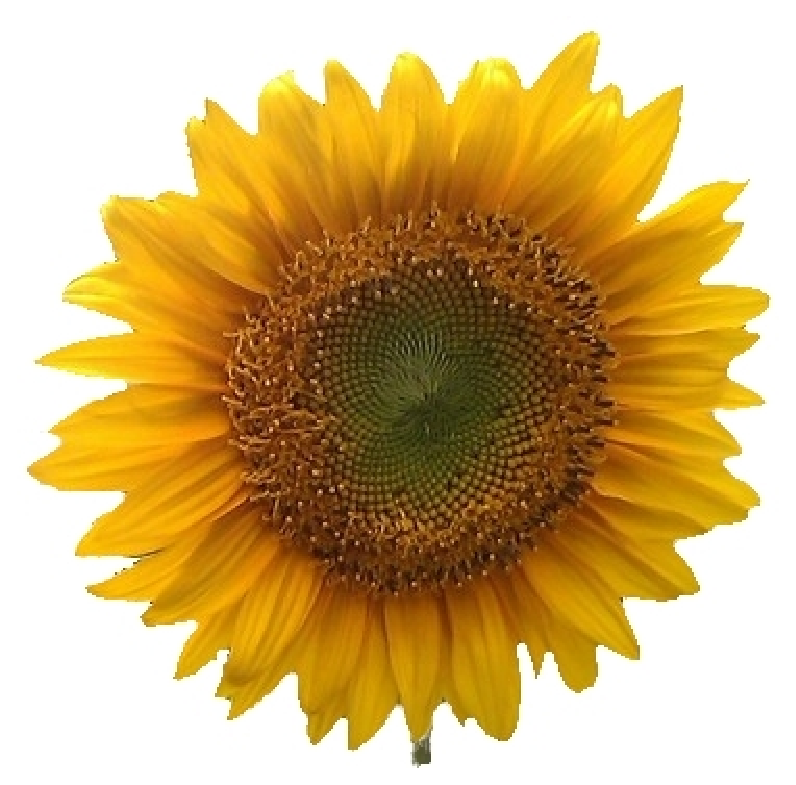
\includegraphics[width=1cm]{sunflower.eps}}
}}

\MNODE(-\XA,0){M}{$B$}
\SF(\XA,0)

\psset{arrows=->,linecolor=darkgray,labelsep=1pt}
\ncarc[arcangle=20]{M}{RR}\aput{0}(0.5){$p$}
\nccircle[angle=90,nodesep=-1pt]{M}{0.3}
\ncarc[arcangle=20]{R}{M}

\end{pspicture}
\endfile
